% Options for packages loaded elsewhere
\PassOptionsToPackage{unicode}{hyperref}
\PassOptionsToPackage{hyphens}{url}
\PassOptionsToPackage{dvipsnames,svgnames,x11names}{xcolor}
%
\documentclass[
  letterpaper,
  DIV=11,
  numbers=noendperiod]{scrartcl}

\usepackage{amsmath,amssymb}
\usepackage{iftex}
\ifPDFTeX
  \usepackage[T1]{fontenc}
  \usepackage[utf8]{inputenc}
  \usepackage{textcomp} % provide euro and other symbols
\else % if luatex or xetex
  \usepackage{unicode-math}
  \defaultfontfeatures{Scale=MatchLowercase}
  \defaultfontfeatures[\rmfamily]{Ligatures=TeX,Scale=1}
\fi
\usepackage{lmodern}
\ifPDFTeX\else  
    % xetex/luatex font selection
\fi
% Use upquote if available, for straight quotes in verbatim environments
\IfFileExists{upquote.sty}{\usepackage{upquote}}{}
\IfFileExists{microtype.sty}{% use microtype if available
  \usepackage[]{microtype}
  \UseMicrotypeSet[protrusion]{basicmath} % disable protrusion for tt fonts
}{}
\makeatletter
\@ifundefined{KOMAClassName}{% if non-KOMA class
  \IfFileExists{parskip.sty}{%
    \usepackage{parskip}
  }{% else
    \setlength{\parindent}{0pt}
    \setlength{\parskip}{6pt plus 2pt minus 1pt}}
}{% if KOMA class
  \KOMAoptions{parskip=half}}
\makeatother
\usepackage{xcolor}
\setlength{\emergencystretch}{3em} % prevent overfull lines
\setcounter{secnumdepth}{-\maxdimen} % remove section numbering
% Make \paragraph and \subparagraph free-standing
\makeatletter
\ifx\paragraph\undefined\else
  \let\oldparagraph\paragraph
  \renewcommand{\paragraph}{
    \@ifstar
      \xxxParagraphStar
      \xxxParagraphNoStar
  }
  \newcommand{\xxxParagraphStar}[1]{\oldparagraph*{#1}\mbox{}}
  \newcommand{\xxxParagraphNoStar}[1]{\oldparagraph{#1}\mbox{}}
\fi
\ifx\subparagraph\undefined\else
  \let\oldsubparagraph\subparagraph
  \renewcommand{\subparagraph}{
    \@ifstar
      \xxxSubParagraphStar
      \xxxSubParagraphNoStar
  }
  \newcommand{\xxxSubParagraphStar}[1]{\oldsubparagraph*{#1}\mbox{}}
  \newcommand{\xxxSubParagraphNoStar}[1]{\oldsubparagraph{#1}\mbox{}}
\fi
\makeatother

\usepackage{color}
\usepackage{fancyvrb}
\newcommand{\VerbBar}{|}
\newcommand{\VERB}{\Verb[commandchars=\\\{\}]}
\DefineVerbatimEnvironment{Highlighting}{Verbatim}{commandchars=\\\{\}}
% Add ',fontsize=\small' for more characters per line
\usepackage{framed}
\definecolor{shadecolor}{RGB}{241,243,245}
\newenvironment{Shaded}{\begin{snugshade}}{\end{snugshade}}
\newcommand{\AlertTok}[1]{\textcolor[rgb]{0.68,0.00,0.00}{#1}}
\newcommand{\AnnotationTok}[1]{\textcolor[rgb]{0.37,0.37,0.37}{#1}}
\newcommand{\AttributeTok}[1]{\textcolor[rgb]{0.40,0.45,0.13}{#1}}
\newcommand{\BaseNTok}[1]{\textcolor[rgb]{0.68,0.00,0.00}{#1}}
\newcommand{\BuiltInTok}[1]{\textcolor[rgb]{0.00,0.23,0.31}{#1}}
\newcommand{\CharTok}[1]{\textcolor[rgb]{0.13,0.47,0.30}{#1}}
\newcommand{\CommentTok}[1]{\textcolor[rgb]{0.37,0.37,0.37}{#1}}
\newcommand{\CommentVarTok}[1]{\textcolor[rgb]{0.37,0.37,0.37}{\textit{#1}}}
\newcommand{\ConstantTok}[1]{\textcolor[rgb]{0.56,0.35,0.01}{#1}}
\newcommand{\ControlFlowTok}[1]{\textcolor[rgb]{0.00,0.23,0.31}{\textbf{#1}}}
\newcommand{\DataTypeTok}[1]{\textcolor[rgb]{0.68,0.00,0.00}{#1}}
\newcommand{\DecValTok}[1]{\textcolor[rgb]{0.68,0.00,0.00}{#1}}
\newcommand{\DocumentationTok}[1]{\textcolor[rgb]{0.37,0.37,0.37}{\textit{#1}}}
\newcommand{\ErrorTok}[1]{\textcolor[rgb]{0.68,0.00,0.00}{#1}}
\newcommand{\ExtensionTok}[1]{\textcolor[rgb]{0.00,0.23,0.31}{#1}}
\newcommand{\FloatTok}[1]{\textcolor[rgb]{0.68,0.00,0.00}{#1}}
\newcommand{\FunctionTok}[1]{\textcolor[rgb]{0.28,0.35,0.67}{#1}}
\newcommand{\ImportTok}[1]{\textcolor[rgb]{0.00,0.46,0.62}{#1}}
\newcommand{\InformationTok}[1]{\textcolor[rgb]{0.37,0.37,0.37}{#1}}
\newcommand{\KeywordTok}[1]{\textcolor[rgb]{0.00,0.23,0.31}{\textbf{#1}}}
\newcommand{\NormalTok}[1]{\textcolor[rgb]{0.00,0.23,0.31}{#1}}
\newcommand{\OperatorTok}[1]{\textcolor[rgb]{0.37,0.37,0.37}{#1}}
\newcommand{\OtherTok}[1]{\textcolor[rgb]{0.00,0.23,0.31}{#1}}
\newcommand{\PreprocessorTok}[1]{\textcolor[rgb]{0.68,0.00,0.00}{#1}}
\newcommand{\RegionMarkerTok}[1]{\textcolor[rgb]{0.00,0.23,0.31}{#1}}
\newcommand{\SpecialCharTok}[1]{\textcolor[rgb]{0.37,0.37,0.37}{#1}}
\newcommand{\SpecialStringTok}[1]{\textcolor[rgb]{0.13,0.47,0.30}{#1}}
\newcommand{\StringTok}[1]{\textcolor[rgb]{0.13,0.47,0.30}{#1}}
\newcommand{\VariableTok}[1]{\textcolor[rgb]{0.07,0.07,0.07}{#1}}
\newcommand{\VerbatimStringTok}[1]{\textcolor[rgb]{0.13,0.47,0.30}{#1}}
\newcommand{\WarningTok}[1]{\textcolor[rgb]{0.37,0.37,0.37}{\textit{#1}}}

\providecommand{\tightlist}{%
  \setlength{\itemsep}{0pt}\setlength{\parskip}{0pt}}\usepackage{longtable,booktabs,array}
\usepackage{calc} % for calculating minipage widths
% Correct order of tables after \paragraph or \subparagraph
\usepackage{etoolbox}
\makeatletter
\patchcmd\longtable{\par}{\if@noskipsec\mbox{}\fi\par}{}{}
\makeatother
% Allow footnotes in longtable head/foot
\IfFileExists{footnotehyper.sty}{\usepackage{footnotehyper}}{\usepackage{footnote}}
\makesavenoteenv{longtable}
\usepackage{graphicx}
\makeatletter
\def\maxwidth{\ifdim\Gin@nat@width>\linewidth\linewidth\else\Gin@nat@width\fi}
\def\maxheight{\ifdim\Gin@nat@height>\textheight\textheight\else\Gin@nat@height\fi}
\makeatother
% Scale images if necessary, so that they will not overflow the page
% margins by default, and it is still possible to overwrite the defaults
% using explicit options in \includegraphics[width, height, ...]{}
\setkeys{Gin}{width=\maxwidth,height=\maxheight,keepaspectratio}
% Set default figure placement to htbp
\makeatletter
\def\fps@figure{htbp}
\makeatother

\usepackage{fvextra}
\DefineVerbatimEnvironment{Highlighting}{Verbatim}{breaklines,commandchars=\\\{\}}
\KOMAoption{captions}{tableheading}
\makeatletter
\@ifpackageloaded{caption}{}{\usepackage{caption}}
\AtBeginDocument{%
\ifdefined\contentsname
  \renewcommand*\contentsname{Table of contents}
\else
  \newcommand\contentsname{Table of contents}
\fi
\ifdefined\listfigurename
  \renewcommand*\listfigurename{List of Figures}
\else
  \newcommand\listfigurename{List of Figures}
\fi
\ifdefined\listtablename
  \renewcommand*\listtablename{List of Tables}
\else
  \newcommand\listtablename{List of Tables}
\fi
\ifdefined\figurename
  \renewcommand*\figurename{Figure}
\else
  \newcommand\figurename{Figure}
\fi
\ifdefined\tablename
  \renewcommand*\tablename{Table}
\else
  \newcommand\tablename{Table}
\fi
}
\@ifpackageloaded{float}{}{\usepackage{float}}
\floatstyle{ruled}
\@ifundefined{c@chapter}{\newfloat{codelisting}{h}{lop}}{\newfloat{codelisting}{h}{lop}[chapter]}
\floatname{codelisting}{Listing}
\newcommand*\listoflistings{\listof{codelisting}{List of Listings}}
\makeatother
\makeatletter
\makeatother
\makeatletter
\@ifpackageloaded{caption}{}{\usepackage{caption}}
\@ifpackageloaded{subcaption}{}{\usepackage{subcaption}}
\makeatother

\ifLuaTeX
  \usepackage{selnolig}  % disable illegal ligatures
\fi
\usepackage{bookmark}

\IfFileExists{xurl.sty}{\usepackage{xurl}}{} % add URL line breaks if available
\urlstyle{same} % disable monospaced font for URLs
\hypersetup{
  pdftitle={Final Project: Reproducible Research},
  pdfauthor={Xinyi Zhou, and Wuzhen Han},
  colorlinks=true,
  linkcolor={blue},
  filecolor={Maroon},
  citecolor={Blue},
  urlcolor={Blue},
  pdfcreator={LaTeX via pandoc}}


\title{Final Project: Reproducible Research}
\author{Xinyi Zhou, and Wuzhen Han}
\date{2024-11-28}

\begin{document}
\maketitle

\RecustomVerbatimEnvironment{verbatim}{Verbatim}{
  showspaces = false,
  showtabs = false,
  breaksymbolleft={},
  breaklines
}


\begin{Shaded}
\begin{Highlighting}[]
\ImportTok{import}\NormalTok{ pandas }\ImportTok{as}\NormalTok{ pd}
\ImportTok{import}\NormalTok{ altair }\ImportTok{as}\NormalTok{ alt}
\ImportTok{import}\NormalTok{ geopandas }\ImportTok{as}\NormalTok{ gpd}
\ImportTok{import}\NormalTok{ json}
\ImportTok{import}\NormalTok{ os}
\ImportTok{from}\NormalTok{ vega\_datasets }\ImportTok{import}\NormalTok{ data}
\ImportTok{import}\NormalTok{ matplotlib.pyplot }\ImportTok{as}\NormalTok{ plt}
\ImportTok{import}\NormalTok{ matplotlib.image }\ImportTok{as}\NormalTok{ mpimg}
\end{Highlighting}
\end{Shaded}

\subsubsection{Merge Data}\label{merge-data}

\begin{Shaded}
\begin{Highlighting}[]
\NormalTok{data\_path }\OperatorTok{=} \StringTok{\textquotesingle{}/Users/cynthia/Desktop/final{-}project{-}xy{-}wz/data\textquotesingle{}}
\NormalTok{real\_gdp\_path }\OperatorTok{=}\NormalTok{ os.path.join(data\_path, }\StringTok{\textquotesingle{}Real\_GDP.csv\textquotesingle{}}\NormalTok{)}
\NormalTok{unemployment\_rate\_path }\OperatorTok{=}\NormalTok{ os.path.join(data\_path, }\StringTok{\textquotesingle{}Unemployment\_rate.csv\textquotesingle{}}\NormalTok{)}

\NormalTok{real\_gdp }\OperatorTok{=}\NormalTok{ pd.read\_csv(real\_gdp\_path)}
\NormalTok{unemployment\_rate }\OperatorTok{=}\NormalTok{ pd.read\_csv(unemployment\_rate\_path)}

\NormalTok{real\_gdp[}\StringTok{\textquotesingle{}DATE\textquotesingle{}}\NormalTok{] }\OperatorTok{=}\NormalTok{ pd.to\_datetime(real\_gdp[}\StringTok{\textquotesingle{}DATE\textquotesingle{}}\NormalTok{])}
\NormalTok{unemployment\_rate[}\StringTok{\textquotesingle{}DATE\textquotesingle{}}\NormalTok{] }\OperatorTok{=}\NormalTok{ pd.to\_datetime(unemployment\_rate[}\StringTok{\textquotesingle{}DATE\textquotesingle{}}\NormalTok{])}

\CommentTok{\# Merge the datasets on the DATE column, keeping all rows from real\_gdp left join}
\NormalTok{merged\_data }\OperatorTok{=}\NormalTok{ pd.merge(real\_gdp, unemployment\_rate, on}\OperatorTok{=}\StringTok{\textquotesingle{}DATE\textquotesingle{}}\NormalTok{, how}\OperatorTok{=}\StringTok{\textquotesingle{}left\textquotesingle{}}\NormalTok{)}

\NormalTok{save\_path }\OperatorTok{=} \StringTok{\textquotesingle{}merged\_data.csv\textquotesingle{}}
\NormalTok{merged\_data.to\_csv(save\_path, index}\OperatorTok{=}\VariableTok{False}\NormalTok{)}
\end{Highlighting}
\end{Shaded}

\subsubsection{Data Preprocessing and Static
graph}\label{data-preprocessing-and-static-graph}

\section{1.Bar chart of state-level CARES Act funding
distribution}\label{bar-chart-of-state-level-cares-act-funding-distribution}

\begin{Shaded}
\begin{Highlighting}[]
\NormalTok{covid\_report\_path }\OperatorTok{=}\NormalTok{ os.path.join(data\_path, }\StringTok{\textquotesingle{}COVID19\_Grant\_Report.csv\textquotesingle{}}\NormalTok{)}
\NormalTok{data\_raw }\OperatorTok{=}\NormalTok{ pd.read\_csv(covid\_report\_path, skiprows}\OperatorTok{=}\DecValTok{5}\NormalTok{)}

\NormalTok{original\_number\_of\_grants }\OperatorTok{=} \BuiltInTok{len}\NormalTok{(data\_raw)}
\BuiltInTok{print}\NormalTok{(}\SpecialStringTok{f"Original Number of Grants: }\SpecialCharTok{\{}\NormalTok{original\_number\_of\_grants}\SpecialCharTok{\}}\SpecialStringTok{"}\NormalTok{)}

\CommentTok{\# Remove dollar signs and commas from Award Funding and convert to float}
\NormalTok{data\_raw[}\StringTok{\textquotesingle{}Award Funding\textquotesingle{}}\NormalTok{] }\OperatorTok{=}\NormalTok{ data\_raw[}\StringTok{\textquotesingle{}Award Funding\textquotesingle{}}\NormalTok{].replace(}
    \VerbatimStringTok{r\textquotesingle{}[$,]\textquotesingle{}}\NormalTok{, }\StringTok{\textquotesingle{}\textquotesingle{}}\NormalTok{, regex}\OperatorTok{=}\VariableTok{True}\NormalTok{).astype(}\BuiltInTok{float}\NormalTok{)}

\NormalTok{converted\_number\_of\_grants }\OperatorTok{=} \BuiltInTok{len}\NormalTok{(data\_raw)}
\BuiltInTok{print}\NormalTok{(}
    \SpecialStringTok{f"Number of Grants after \textquotesingle{}Award Funding\textquotesingle{} conversion: }\SpecialCharTok{\{}\NormalTok{converted\_number\_of\_grants}\SpecialCharTok{\}}\SpecialStringTok{"}\NormalTok{)}

\NormalTok{data\_cleaned }\OperatorTok{=}\NormalTok{ data\_raw.dropna(subset}\OperatorTok{=}\NormalTok{[}\StringTok{\textquotesingle{}State\textquotesingle{}}\NormalTok{, }\StringTok{\textquotesingle{}Award Funding\textquotesingle{}}\NormalTok{])}
\BuiltInTok{print}\NormalTok{(}\SpecialStringTok{f"Number of Grants after dropping NaNs: }\SpecialCharTok{\{}\BuiltInTok{len}\NormalTok{(data\_cleaned)}\SpecialCharTok{\}}\SpecialStringTok{"}\NormalTok{)}

\NormalTok{total\_funding\_dollars }\OperatorTok{=}\NormalTok{ data\_cleaned[}\StringTok{\textquotesingle{}Award Funding\textquotesingle{}}\NormalTok{].}\BuiltInTok{sum}\NormalTok{()}
\BuiltInTok{print}\NormalTok{(}
    \SpecialStringTok{f"Total Award Funding for all grants (Dollars): }\SpecialCharTok{\{}\NormalTok{total\_funding\_dollars}\SpecialCharTok{:,.0f\}}\SpecialStringTok{"}\NormalTok{)}

\CommentTok{\# Group by State and sum the Award Funding, converting to millions}
\NormalTok{state\_funding }\OperatorTok{=}\NormalTok{ data\_cleaned.groupby(}
    \StringTok{\textquotesingle{}State\textquotesingle{}}\NormalTok{)[}\StringTok{\textquotesingle{}Award Funding\textquotesingle{}}\NormalTok{].}\BuiltInTok{sum}\NormalTok{().reset\_index()}

\NormalTok{state\_funding[}\StringTok{\textquotesingle{}Award Funding\textquotesingle{}}\NormalTok{] }\OperatorTok{=}\NormalTok{ state\_funding[}\StringTok{\textquotesingle{}Award Funding\textquotesingle{}}\NormalTok{] }\OperatorTok{/} \FloatTok{1e6}

\CommentTok{\# Sort states by funding amount in descending order}
\NormalTok{state\_funding }\OperatorTok{=}\NormalTok{ state\_funding.sort\_values(}
\NormalTok{    by}\OperatorTok{=}\StringTok{\textquotesingle{}Award Funding\textquotesingle{}}\NormalTok{, ascending}\OperatorTok{=}\VariableTok{False}\NormalTok{).reset\_index(drop}\OperatorTok{=}\VariableTok{True}\NormalTok{)}

\NormalTok{chart }\OperatorTok{=}\NormalTok{ alt.Chart(state\_funding).mark\_bar(color}\OperatorTok{=}\StringTok{\textquotesingle{}skyblue\textquotesingle{}}\NormalTok{).encode(}
\NormalTok{    y}\OperatorTok{=}\NormalTok{alt.Y(}\StringTok{\textquotesingle{}State:N\textquotesingle{}}\NormalTok{, sort}\OperatorTok{=}\StringTok{\textquotesingle{}{-}x\textquotesingle{}}\NormalTok{, title}\OperatorTok{=}\StringTok{\textquotesingle{}State\textquotesingle{}}\NormalTok{),}
\NormalTok{    x}\OperatorTok{=}\NormalTok{alt.X(}\StringTok{\textquotesingle{}Award Funding:Q\textquotesingle{}}\NormalTok{, title}\OperatorTok{=}\StringTok{\textquotesingle{}Total Award Funding (Millions $)\textquotesingle{}}\NormalTok{),}
\NormalTok{    tooltip}\OperatorTok{=}\NormalTok{[}\StringTok{\textquotesingle{}State\textquotesingle{}}\NormalTok{, }\StringTok{\textquotesingle{}Award Funding\textquotesingle{}}\NormalTok{]}
\NormalTok{).properties(}
\NormalTok{    title}\OperatorTok{=}\StringTok{\textquotesingle{}Total Funding Amount by State\textquotesingle{}}\NormalTok{,}
\NormalTok{    width}\OperatorTok{=}\DecValTok{600}\NormalTok{,}
\NormalTok{    height}\OperatorTok{=}\DecValTok{500}
\NormalTok{).configure\_axis(}
\NormalTok{    labelAngle}\OperatorTok{=}\DecValTok{0}
\NormalTok{)}

\BuiltInTok{print}\NormalTok{(}\StringTok{"Top 3 states with the highest funding (in millions):"}\NormalTok{)}
\BuiltInTok{print}\NormalTok{(state\_funding.head(}\DecValTok{3}\NormalTok{))}

\NormalTok{chart}
\end{Highlighting}
\end{Shaded}

\begin{verbatim}
Original Number of Grants: 1389
Number of Grants after 'Award Funding' conversion: 1389
Number of Grants after dropping NaNs: 1387
Total Award Funding for all grants (Dollars): 1,316,374,135
Top 3 states with the highest funding (in millions):
  State  Award Funding
0    CA     193.072106
1    TX      76.701360
2    NY      76.696605
\end{verbatim}

\begin{verbatim}
alt.Chart(...)
\end{verbatim}

\section{2. Economic Trends During COVID-19: Real GDP and Unemployment
Rate
(2018--2024)}\label{economic-trends-during-covid-19-real-gdp-and-unemployment-rate-20182024}

\begin{Shaded}
\begin{Highlighting}[]
\CommentTok{\# Create a line chart for Real GDP}
\NormalTok{gdp\_chart }\OperatorTok{=}\NormalTok{ alt.Chart(merged\_data).mark\_line(color}\OperatorTok{=}\StringTok{\textquotesingle{}blue\textquotesingle{}}\NormalTok{).encode(}
\NormalTok{    alt.X(}\StringTok{\textquotesingle{}DATE:T\textquotesingle{}}\NormalTok{, title}\OperatorTok{=}\StringTok{\textquotesingle{}Date\textquotesingle{}}\NormalTok{, axis}\OperatorTok{=}\NormalTok{alt.Axis(}\BuiltInTok{format}\OperatorTok{=}\StringTok{\textquotesingle{}\%Y/\%m/}\SpecialCharTok{\%d}\StringTok{\textquotesingle{}}\NormalTok{, grid}\OperatorTok{=}\VariableTok{False}\NormalTok{)),}
\NormalTok{    alt.Y(}\StringTok{\textquotesingle{}GDPC1:Q\textquotesingle{}}\NormalTok{, title}\OperatorTok{=}\StringTok{\textquotesingle{}Real GDP (Billion $)\textquotesingle{}}\NormalTok{, axis}\OperatorTok{=}\NormalTok{alt.Axis(grid}\OperatorTok{=}\VariableTok{False}\NormalTok{),}
\NormalTok{          scale}\OperatorTok{=}\NormalTok{alt.Scale(domain}\OperatorTok{=}\NormalTok{[merged\_data[}\StringTok{\textquotesingle{}GDPC1\textquotesingle{}}\NormalTok{].}\BuiltInTok{min}\NormalTok{(), merged\_data[}\StringTok{\textquotesingle{}GDPC1\textquotesingle{}}\NormalTok{].}\BuiltInTok{max}\NormalTok{()]))}
\NormalTok{)}

\CommentTok{\# Create a line chart for Unemployment Rate}
\NormalTok{unrate\_chart }\OperatorTok{=}\NormalTok{ alt.Chart(merged\_data).mark\_line(color}\OperatorTok{=}\StringTok{\textquotesingle{}orange\textquotesingle{}}\NormalTok{).encode(}
\NormalTok{    alt.X(}\StringTok{\textquotesingle{}DATE:T\textquotesingle{}}\NormalTok{, title}\OperatorTok{=}\StringTok{\textquotesingle{}Date\textquotesingle{}}\NormalTok{, axis}\OperatorTok{=}\NormalTok{alt.Axis(}\BuiltInTok{format}\OperatorTok{=}\StringTok{\textquotesingle{}\%Y/\%m/}\SpecialCharTok{\%d}\StringTok{\textquotesingle{}}\NormalTok{, grid}\OperatorTok{=}\VariableTok{False}\NormalTok{)),}
\NormalTok{    alt.Y(}\StringTok{\textquotesingle{}UNRATE:Q\textquotesingle{}}\NormalTok{, title}\OperatorTok{=}\StringTok{\textquotesingle{}Unemployment Rate (\%)\textquotesingle{}}\NormalTok{, axis}\OperatorTok{=}\NormalTok{alt.Axis(}
\NormalTok{        grid}\OperatorTok{=}\VariableTok{False}\NormalTok{), scale}\OperatorTok{=}\NormalTok{alt.Scale(domain}\OperatorTok{=}\NormalTok{[}\DecValTok{0}\NormalTok{, merged\_data[}\StringTok{\textquotesingle{}UNRATE\textquotesingle{}}\NormalTok{].}\BuiltInTok{max}\NormalTok{()]))}
\NormalTok{).properties(}
\NormalTok{    title}\OperatorTok{=}\StringTok{"Time Trends: Real GDP and Unemployment Rate (2018–2024)"}
\NormalTok{)}

\CommentTok{\# Layer both charts together and resolve independent y{-}scales}
\NormalTok{chart }\OperatorTok{=}\NormalTok{ alt.layer(}
\NormalTok{    gdp\_chart, unrate\_chart}
\NormalTok{).resolve\_scale(}
\NormalTok{    y}\OperatorTok{=}\StringTok{\textquotesingle{}independent\textquotesingle{}}
\NormalTok{).properties(}
\NormalTok{    width}\OperatorTok{=}\DecValTok{800}\NormalTok{,}
\NormalTok{    height}\OperatorTok{=}\DecValTok{400}
\NormalTok{)}

\NormalTok{chart.show()}
\end{Highlighting}
\end{Shaded}

\begin{verbatim}
alt.LayerChart(...)
\end{verbatim}

\section{3. State-Level Unemployment Rate: Dynamic Heatmap by
Time}\label{state-level-unemployment-rate-dynamic-heatmap-by-time}

\subsection{getting data}\label{getting-data}

\section{Download the required unemployment rate
documentation(https://dlt.ri.gov/media/15101/download?language=en).It
is then processed manually to extract key information from the file,
such as the year, state name,
etc}\label{download-the-required-unemployment-rate-documentationhttpsdlt.ri.govmedia15101downloadlanguageen.it-is-then-processed-manually-to-extract-key-information-from-the-file-such-as-the-year-state-name-etc}

\section{a. Create static maps of unemployment rates by
state}\label{a.-create-static-maps-of-unemployment-rates-by-state}

\section{2024}\label{section}

\begin{Shaded}
\begin{Highlighting}[]
\NormalTok{unemp\_state }\OperatorTok{=}\NormalTok{ os.path.join(data\_path, }\StringTok{\textquotesingle{}anunemp.csv\textquotesingle{}}\NormalTok{)}
\NormalTok{unemployment\_data }\OperatorTok{=}\NormalTok{ pd.read\_csv(unemp\_state)}

\NormalTok{unemployment\_data\_filtered }\OperatorTok{=}\NormalTok{ unemployment\_data.loc[unemployment\_data[}\StringTok{\textquotesingle{}State\textquotesingle{}}\NormalTok{] }\OperatorTok{!=} \StringTok{"United States"}\NormalTok{].copy(}
\NormalTok{)}
\NormalTok{unemployment\_data\_filtered[}\StringTok{\textquotesingle{}State\textquotesingle{}}\NormalTok{] }\OperatorTok{=}\NormalTok{ unemployment\_data\_filtered[}\StringTok{\textquotesingle{}State\textquotesingle{}}\NormalTok{].}\BuiltInTok{str}\NormalTok{.strip(}
\NormalTok{).}\BuiltInTok{str}\NormalTok{.title()}

\NormalTok{data\_path\_shp }\OperatorTok{=} \StringTok{\textquotesingle{}/Users/cynthia/Desktop/final{-}project{-}xy{-}wz/cb\_2018\_us\_state\_500k\textquotesingle{}}
\NormalTok{shapefile\_path }\OperatorTok{=}\NormalTok{ os.path.join(data\_path\_shp, }\StringTok{\textquotesingle{}cb\_2018\_us\_state\_500k.shp\textquotesingle{}}\NormalTok{)}
\NormalTok{gdf\_states }\OperatorTok{=}\NormalTok{ gpd.read\_file(shapefile\_path)}

\NormalTok{gdf\_states[}\StringTok{\textquotesingle{}NAME\textquotesingle{}}\NormalTok{] }\OperatorTok{=}\NormalTok{ gdf\_states[}\StringTok{\textquotesingle{}NAME\textquotesingle{}}\NormalTok{].}\BuiltInTok{str}\NormalTok{.strip().}\BuiltInTok{str}\NormalTok{.title()}

\NormalTok{gdf\_merged }\OperatorTok{=}\NormalTok{ gdf\_states.merge(}
\NormalTok{    unemployment\_data\_filtered, how}\OperatorTok{=}\StringTok{\textquotesingle{}left\textquotesingle{}}\NormalTok{, left\_on}\OperatorTok{=}\StringTok{\textquotesingle{}NAME\textquotesingle{}}\NormalTok{, right\_on}\OperatorTok{=}\StringTok{\textquotesingle{}State\textquotesingle{}}
\NormalTok{)}
\NormalTok{gdf\_merged[}\StringTok{\textquotesingle{}Rate\_2024\textquotesingle{}}\NormalTok{] }\OperatorTok{=}\NormalTok{ gdf\_merged[}\StringTok{\textquotesingle{}Rate\_2024\textquotesingle{}}\NormalTok{].fillna(}\DecValTok{0}\NormalTok{)}

\NormalTok{geojson }\OperatorTok{=}\NormalTok{ gdf\_merged.to\_json()}
\NormalTok{geojson\_data }\OperatorTok{=}\NormalTok{ json.loads(geojson)}

\NormalTok{states }\OperatorTok{=}\NormalTok{ alt.Data(values}\OperatorTok{=}\NormalTok{geojson\_data[}\StringTok{\textquotesingle{}features\textquotesingle{}}\NormalTok{])}

\NormalTok{unemployment\_chart }\OperatorTok{=}\NormalTok{ alt.Chart(states).mark\_geoshape(}
\NormalTok{    stroke}\OperatorTok{=}\StringTok{\textquotesingle{}black\textquotesingle{}}\NormalTok{,}
\NormalTok{    strokeWidth}\OperatorTok{=}\DecValTok{1}
\NormalTok{).encode(}
\NormalTok{    color}\OperatorTok{=}\NormalTok{alt.Color(}\StringTok{\textquotesingle{}properties.Rate\_2024:Q\textquotesingle{}}\NormalTok{,}
\NormalTok{                    scale}\OperatorTok{=}\NormalTok{alt.Scale(domain}\OperatorTok{=}\NormalTok{[}\DecValTok{0}\NormalTok{, }\DecValTok{10}\NormalTok{], scheme}\OperatorTok{=}\StringTok{\textquotesingle{}orangered\textquotesingle{}}\NormalTok{),}
\NormalTok{                    title}\OperatorTok{=}\StringTok{\textquotesingle{}Unemployment Rate in 2024 (\%)\textquotesingle{}}\NormalTok{),}
\NormalTok{    tooltip}\OperatorTok{=}\NormalTok{[}
\NormalTok{        alt.Tooltip(}\StringTok{\textquotesingle{}properties.NAME:N\textquotesingle{}}\NormalTok{, title}\OperatorTok{=}\StringTok{\textquotesingle{}State\textquotesingle{}}\NormalTok{),}
\NormalTok{        alt.Tooltip(}\StringTok{\textquotesingle{}properties.Rate\_2024:Q\textquotesingle{}}\NormalTok{, title}\OperatorTok{=}\StringTok{\textquotesingle{}Unemployment Rate (\%)\textquotesingle{}}\NormalTok{)}
\NormalTok{    ]}
\NormalTok{).project(}
    \BuiltInTok{type}\OperatorTok{=}\StringTok{\textquotesingle{}albersUsa\textquotesingle{}}
\NormalTok{).properties(}
\NormalTok{    width}\OperatorTok{=}\DecValTok{500}\NormalTok{,}
\NormalTok{    height}\OperatorTok{=}\DecValTok{500}\NormalTok{,}
\NormalTok{    title}\OperatorTok{=}\StringTok{\textquotesingle{}Unemployment Rate by State (2024)\textquotesingle{}}
\NormalTok{)}

\NormalTok{unemployment\_chart.display()}

\NormalTok{top\_3\_states }\OperatorTok{=}\NormalTok{ gdf\_merged.nlargest(}\DecValTok{3}\NormalTok{, }\StringTok{\textquotesingle{}Rate\_2024\textquotesingle{}}\NormalTok{)[[}\StringTok{\textquotesingle{}NAME\textquotesingle{}}\NormalTok{, }\StringTok{\textquotesingle{}Rate\_2024\textquotesingle{}}\NormalTok{]]}
\BuiltInTok{print}\NormalTok{(top\_3\_states)}
\end{Highlighting}
\end{Shaded}

\begin{verbatim}
alt.Chart(...)
\end{verbatim}

\begin{verbatim}
                    NAME  Rate_2024
28                Nevada        5.7
36  District Of Columbia        5.7
16            California        5.4
\end{verbatim}

\section{2023}\label{section-1}

\begin{Shaded}
\begin{Highlighting}[]
\NormalTok{gdf\_merged\_2023 }\OperatorTok{=}\NormalTok{ gdf\_states.merge(}
\NormalTok{    unemployment\_data\_filtered, how}\OperatorTok{=}\StringTok{\textquotesingle{}left\textquotesingle{}}\NormalTok{, left\_on}\OperatorTok{=}\StringTok{\textquotesingle{}NAME\textquotesingle{}}\NormalTok{, right\_on}\OperatorTok{=}\StringTok{\textquotesingle{}State\textquotesingle{}}
\NormalTok{)}
\NormalTok{gdf\_merged\_2023[}\StringTok{\textquotesingle{}Rate\_2023\textquotesingle{}}\NormalTok{] }\OperatorTok{=}\NormalTok{ gdf\_merged\_2023[}\StringTok{\textquotesingle{}Rate\_2023\textquotesingle{}}\NormalTok{].fillna(}\DecValTok{0}\NormalTok{)}

\NormalTok{geojson }\OperatorTok{=}\NormalTok{ gdf\_merged\_2023.to\_json()}
\NormalTok{geojson\_data }\OperatorTok{=}\NormalTok{ json.loads(geojson)}

\NormalTok{states }\OperatorTok{=}\NormalTok{ alt.Data(values}\OperatorTok{=}\NormalTok{geojson\_data[}\StringTok{\textquotesingle{}features\textquotesingle{}}\NormalTok{])}

\NormalTok{unemployment\_chart\_2023 }\OperatorTok{=}\NormalTok{ alt.Chart(states).mark\_geoshape(}
\NormalTok{    stroke}\OperatorTok{=}\StringTok{\textquotesingle{}black\textquotesingle{}}\NormalTok{,}
\NormalTok{    strokeWidth}\OperatorTok{=}\DecValTok{1}
\NormalTok{).encode(}
\NormalTok{    color}\OperatorTok{=}\NormalTok{alt.Color(}\StringTok{\textquotesingle{}properties.Rate\_2023:Q\textquotesingle{}}\NormalTok{,}
\NormalTok{                    scale}\OperatorTok{=}\NormalTok{alt.Scale(domain}\OperatorTok{=}\NormalTok{[}\DecValTok{0}\NormalTok{, }\DecValTok{10}\NormalTok{], scheme}\OperatorTok{=}\StringTok{\textquotesingle{}orangered\textquotesingle{}}\NormalTok{),}
\NormalTok{                    title}\OperatorTok{=}\StringTok{\textquotesingle{}Unemployment Rate in 2023 (\%)\textquotesingle{}}\NormalTok{),}
\NormalTok{    tooltip}\OperatorTok{=}\NormalTok{[}
\NormalTok{        alt.Tooltip(}\StringTok{\textquotesingle{}properties.NAME:N\textquotesingle{}}\NormalTok{, title}\OperatorTok{=}\StringTok{\textquotesingle{}State\textquotesingle{}}\NormalTok{),}
\NormalTok{        alt.Tooltip(}\StringTok{\textquotesingle{}properties.Rate\_2023:Q\textquotesingle{}}\NormalTok{, title}\OperatorTok{=}\StringTok{\textquotesingle{}Unemployment Rate (\%)\textquotesingle{}}\NormalTok{)}
\NormalTok{    ]}
\NormalTok{).project(}
    \BuiltInTok{type}\OperatorTok{=}\StringTok{\textquotesingle{}albersUsa\textquotesingle{}}
\NormalTok{).properties(}
\NormalTok{    width}\OperatorTok{=}\DecValTok{500}\NormalTok{,}
\NormalTok{    height}\OperatorTok{=}\DecValTok{500}\NormalTok{,}
\NormalTok{    title}\OperatorTok{=}\StringTok{\textquotesingle{}Unemployment Rate by State (2023)\textquotesingle{}}
\NormalTok{)}

\NormalTok{unemployment\_chart\_2023.display()}

\NormalTok{top\_3\_states\_2023 }\OperatorTok{=}\NormalTok{ gdf\_merged\_2023.nlargest(}
    \DecValTok{3}\NormalTok{, }\StringTok{\textquotesingle{}Rate\_2023\textquotesingle{}}\NormalTok{)[[}\StringTok{\textquotesingle{}NAME\textquotesingle{}}\NormalTok{, }\StringTok{\textquotesingle{}Rate\_2023\textquotesingle{}}\NormalTok{]]}
\BuiltInTok{print}\NormalTok{(top\_3\_states\_2023)}
\end{Highlighting}
\end{Shaded}

\begin{verbatim}
alt.Chart(...)
\end{verbatim}

\begin{verbatim}
          NAME  Rate_2023
28      Nevada        5.3
29    Illinois        5.3
16  California        5.1
\end{verbatim}

\section{2022}\label{section-2}

\begin{Shaded}
\begin{Highlighting}[]
\NormalTok{gdf\_merged\_2022 }\OperatorTok{=}\NormalTok{ gdf\_states.merge(}
\NormalTok{    unemployment\_data\_filtered, how}\OperatorTok{=}\StringTok{\textquotesingle{}left\textquotesingle{}}\NormalTok{, left\_on}\OperatorTok{=}\StringTok{\textquotesingle{}NAME\textquotesingle{}}\NormalTok{, right\_on}\OperatorTok{=}\StringTok{\textquotesingle{}State\textquotesingle{}}
\NormalTok{)}
\NormalTok{gdf\_merged\_2022[}\StringTok{\textquotesingle{}Rate\_2022\textquotesingle{}}\NormalTok{] }\OperatorTok{=}\NormalTok{ gdf\_merged\_2022[}\StringTok{\textquotesingle{}Rate\_2022\textquotesingle{}}\NormalTok{].fillna(}\DecValTok{0}\NormalTok{)}

\NormalTok{geojson\_2022 }\OperatorTok{=}\NormalTok{ gdf\_merged\_2022.to\_json()}
\NormalTok{geojson\_data\_2022 }\OperatorTok{=}\NormalTok{ json.loads(geojson\_2022)}

\NormalTok{states\_2022 }\OperatorTok{=}\NormalTok{ alt.Data(values}\OperatorTok{=}\NormalTok{geojson\_data\_2022[}\StringTok{\textquotesingle{}features\textquotesingle{}}\NormalTok{])}

\NormalTok{unemployment\_chart\_2022 }\OperatorTok{=}\NormalTok{ alt.Chart(states\_2022).mark\_geoshape(}
\NormalTok{    stroke}\OperatorTok{=}\StringTok{\textquotesingle{}black\textquotesingle{}}\NormalTok{,}
\NormalTok{    strokeWidth}\OperatorTok{=}\DecValTok{1}
\NormalTok{).encode(}
\NormalTok{    color}\OperatorTok{=}\NormalTok{alt.Color(}\StringTok{\textquotesingle{}properties.Rate\_2022:Q\textquotesingle{}}\NormalTok{, }
\NormalTok{                    scale}\OperatorTok{=}\NormalTok{alt.Scale(domain}\OperatorTok{=}\NormalTok{[}\DecValTok{0}\NormalTok{, }\DecValTok{10}\NormalTok{], scheme}\OperatorTok{=}\StringTok{\textquotesingle{}orangered\textquotesingle{}}\NormalTok{),}
\NormalTok{                    title}\OperatorTok{=}\StringTok{\textquotesingle{}Unemployment Rate in 2022 (\%)\textquotesingle{}}\NormalTok{),}
\NormalTok{    tooltip}\OperatorTok{=}\NormalTok{[}
\NormalTok{        alt.Tooltip(}\StringTok{\textquotesingle{}properties.NAME:N\textquotesingle{}}\NormalTok{, title}\OperatorTok{=}\StringTok{\textquotesingle{}State\textquotesingle{}}\NormalTok{),}
\NormalTok{        alt.Tooltip(}\StringTok{\textquotesingle{}properties.Rate\_2022:Q\textquotesingle{}}\NormalTok{, title}\OperatorTok{=}\StringTok{\textquotesingle{}Unemployment Rate (\%)\textquotesingle{}}\NormalTok{)}
\NormalTok{    ]}
\NormalTok{).project(}
    \BuiltInTok{type}\OperatorTok{=}\StringTok{\textquotesingle{}albersUsa\textquotesingle{}}  
\NormalTok{).properties(}
\NormalTok{    width}\OperatorTok{=}\DecValTok{500}\NormalTok{,}
\NormalTok{    height}\OperatorTok{=}\DecValTok{500}\NormalTok{,}
\NormalTok{    title}\OperatorTok{=}\StringTok{\textquotesingle{}Unemployment Rate by State (2022)\textquotesingle{}}
\NormalTok{)}

\NormalTok{unemployment\_chart\_2022.display()}

\NormalTok{top\_3\_states\_2022 }\OperatorTok{=}\NormalTok{ gdf\_merged\_2022.nlargest(}\DecValTok{3}\NormalTok{, }\StringTok{\textquotesingle{}Rate\_2022\textquotesingle{}}\NormalTok{)[[}\StringTok{\textquotesingle{}NAME\textquotesingle{}}\NormalTok{, }\StringTok{\textquotesingle{}Rate\_2022\textquotesingle{}}\NormalTok{]]}
\BuiltInTok{print}\NormalTok{(top\_3\_states\_2022)}
\end{Highlighting}
\end{Shaded}

\begin{verbatim}
alt.Chart(...)
\end{verbatim}

\begin{verbatim}
                    NAME  Rate_2022
28                Nevada        5.2
36  District Of Columbia        4.7
29              Illinois        4.6
\end{verbatim}

\section{2021}\label{section-3}

\begin{Shaded}
\begin{Highlighting}[]
\NormalTok{gdf\_merged\_2021 }\OperatorTok{=}\NormalTok{ gdf\_states.merge(}
\NormalTok{    unemployment\_data\_filtered, how}\OperatorTok{=}\StringTok{\textquotesingle{}left\textquotesingle{}}\NormalTok{, left\_on}\OperatorTok{=}\StringTok{\textquotesingle{}NAME\textquotesingle{}}\NormalTok{, right\_on}\OperatorTok{=}\StringTok{\textquotesingle{}State\textquotesingle{}}\NormalTok{)}
\NormalTok{gdf\_merged\_2021[}\StringTok{\textquotesingle{}Rate\_2021\textquotesingle{}}\NormalTok{] }\OperatorTok{=}\NormalTok{ gdf\_merged\_2021[}\StringTok{\textquotesingle{}Rate\_2021\textquotesingle{}}\NormalTok{].fillna(}\DecValTok{0}\NormalTok{)}

\NormalTok{geojson\_2021 }\OperatorTok{=}\NormalTok{ gdf\_merged\_2021.to\_json()}
\NormalTok{geojson\_data\_2021 }\OperatorTok{=}\NormalTok{ json.loads(geojson\_2021)}

\NormalTok{states\_2021 }\OperatorTok{=}\NormalTok{ alt.Data(values}\OperatorTok{=}\NormalTok{geojson\_data\_2021[}\StringTok{\textquotesingle{}features\textquotesingle{}}\NormalTok{])}

\NormalTok{unemployment\_chart\_2021 }\OperatorTok{=}\NormalTok{ alt.Chart(states\_2021).mark\_geoshape(}
\NormalTok{    stroke}\OperatorTok{=}\StringTok{\textquotesingle{}black\textquotesingle{}}\NormalTok{,}
\NormalTok{    strokeWidth}\OperatorTok{=}\DecValTok{1}
\NormalTok{).encode(}
\NormalTok{    color}\OperatorTok{=}\NormalTok{alt.Color(}\StringTok{\textquotesingle{}properties.Rate\_2021:Q\textquotesingle{}}\NormalTok{,}
\NormalTok{                    scale}\OperatorTok{=}\NormalTok{alt.Scale(domain}\OperatorTok{=}\NormalTok{[}\DecValTok{0}\NormalTok{, }\DecValTok{10}\NormalTok{], scheme}\OperatorTok{=}\StringTok{\textquotesingle{}orangered\textquotesingle{}}\NormalTok{),}
\NormalTok{                    title}\OperatorTok{=}\StringTok{\textquotesingle{}Unemployment Rate in 2021 (\%)\textquotesingle{}}\NormalTok{),}
\NormalTok{    tooltip}\OperatorTok{=}\NormalTok{[}
\NormalTok{        alt.Tooltip(}\StringTok{\textquotesingle{}properties.NAME:N\textquotesingle{}}\NormalTok{, title}\OperatorTok{=}\StringTok{\textquotesingle{}State\textquotesingle{}}\NormalTok{),}
\NormalTok{        alt.Tooltip(}\StringTok{\textquotesingle{}properties.Rate\_2021:Q\textquotesingle{}}\NormalTok{, title}\OperatorTok{=}\StringTok{\textquotesingle{}Unemployment Rate (\%)\textquotesingle{}}\NormalTok{)}
\NormalTok{    ]}
\NormalTok{).project(}
    \BuiltInTok{type}\OperatorTok{=}\StringTok{\textquotesingle{}albersUsa\textquotesingle{}}
\NormalTok{).properties(}
\NormalTok{    width}\OperatorTok{=}\DecValTok{500}\NormalTok{,}
\NormalTok{    height}\OperatorTok{=}\DecValTok{500}\NormalTok{,}
\NormalTok{    title}\OperatorTok{=}\StringTok{\textquotesingle{}Unemployment Rate by State (2021)\textquotesingle{}}
\NormalTok{)}

\NormalTok{unemployment\_chart\_2021.display()}

\NormalTok{top\_3\_states\_2021 }\OperatorTok{=}\NormalTok{ gdf\_merged\_2021.nlargest(}
    \DecValTok{3}\NormalTok{, }\StringTok{\textquotesingle{}Rate\_2021\textquotesingle{}}\NormalTok{)[[}\StringTok{\textquotesingle{}NAME\textquotesingle{}}\NormalTok{, }\StringTok{\textquotesingle{}Rate\_2021\textquotesingle{}}\NormalTok{]]}
\BuiltInTok{print}\NormalTok{(top\_3\_states\_2021)}
\end{Highlighting}
\end{Shaded}

\begin{verbatim}
alt.Chart(...)
\end{verbatim}

\begin{verbatim}
          NAME  Rate_2021
16  California        7.3
12  New Mexico        7.1
25    New York        7.1
\end{verbatim}

\section{2020,2019,2018}\label{section-4}

\begin{Shaded}
\begin{Highlighting}[]
\NormalTok{gdf\_merged\_2020 }\OperatorTok{=}\NormalTok{ gdf\_states.merge(}
\NormalTok{    unemployment\_data\_filtered, how}\OperatorTok{=}\StringTok{\textquotesingle{}left\textquotesingle{}}\NormalTok{, left\_on}\OperatorTok{=}\StringTok{\textquotesingle{}NAME\textquotesingle{}}\NormalTok{, right\_on}\OperatorTok{=}\StringTok{\textquotesingle{}State\textquotesingle{}}\NormalTok{).copy()}
\NormalTok{gdf\_merged\_2020[}\StringTok{\textquotesingle{}Rate\_2020\textquotesingle{}}\NormalTok{] }\OperatorTok{=}\NormalTok{ gdf\_merged\_2020[}\StringTok{\textquotesingle{}Rate\_2020\textquotesingle{}}\NormalTok{].fillna(}\DecValTok{0}\NormalTok{)}

\NormalTok{geojson\_2020 }\OperatorTok{=}\NormalTok{ gdf\_merged\_2020.to\_json()}
\NormalTok{geojson\_data\_2020 }\OperatorTok{=}\NormalTok{ json.loads(geojson\_2020)}

\NormalTok{states\_2020 }\OperatorTok{=}\NormalTok{ alt.Data(values}\OperatorTok{=}\NormalTok{geojson\_data\_2020[}\StringTok{\textquotesingle{}features\textquotesingle{}}\NormalTok{])}

\NormalTok{unemployment\_chart\_2020 }\OperatorTok{=}\NormalTok{ alt.Chart(states\_2020).mark\_geoshape(}
\NormalTok{    stroke}\OperatorTok{=}\StringTok{\textquotesingle{}black\textquotesingle{}}\NormalTok{,}
\NormalTok{    strokeWidth}\OperatorTok{=}\DecValTok{1}
\NormalTok{).encode(}
\NormalTok{    color}\OperatorTok{=}\NormalTok{alt.Color(}\StringTok{\textquotesingle{}properties.Rate\_2020:Q\textquotesingle{}}\NormalTok{,}
\NormalTok{                    scale}\OperatorTok{=}\NormalTok{alt.Scale(domain}\OperatorTok{=}\NormalTok{[}\DecValTok{0}\NormalTok{, }\DecValTok{10}\NormalTok{], scheme}\OperatorTok{=}\StringTok{\textquotesingle{}orangered\textquotesingle{}}\NormalTok{),}
\NormalTok{                    title}\OperatorTok{=}\StringTok{\textquotesingle{}Unemployment Rate in 2020 (\%)\textquotesingle{}}\NormalTok{),}
\NormalTok{    tooltip}\OperatorTok{=}\NormalTok{[}
\NormalTok{        alt.Tooltip(}\StringTok{\textquotesingle{}properties.NAME:N\textquotesingle{}}\NormalTok{, title}\OperatorTok{=}\StringTok{\textquotesingle{}State\textquotesingle{}}\NormalTok{),}
\NormalTok{        alt.Tooltip(}\StringTok{\textquotesingle{}properties.Rate\_2020:Q\textquotesingle{}}\NormalTok{, title}\OperatorTok{=}\StringTok{\textquotesingle{}Unemployment Rate (\%)\textquotesingle{}}\NormalTok{)}
\NormalTok{    ]}
\NormalTok{).project(}
    \BuiltInTok{type}\OperatorTok{=}\StringTok{\textquotesingle{}albersUsa\textquotesingle{}}
\NormalTok{).properties(}
\NormalTok{    width}\OperatorTok{=}\DecValTok{500}\NormalTok{,}
\NormalTok{    height}\OperatorTok{=}\DecValTok{500}\NormalTok{,}
\NormalTok{    title}\OperatorTok{=}\StringTok{\textquotesingle{}Unemployment Rate by State (2020)\textquotesingle{}}
\NormalTok{)}

\NormalTok{unemployment\_chart\_2020.display()}

\NormalTok{top\_3\_states\_2020 }\OperatorTok{=}\NormalTok{ gdf\_merged\_2020.nlargest(}
    \DecValTok{3}\NormalTok{, }\StringTok{\textquotesingle{}Rate\_2020\textquotesingle{}}\NormalTok{)[[}\StringTok{\textquotesingle{}NAME\textquotesingle{}}\NormalTok{, }\StringTok{\textquotesingle{}Rate\_2020\textquotesingle{}}\NormalTok{]]}
\BuiltInTok{print}\NormalTok{(top\_3\_states\_2020)}

\NormalTok{gdf\_merged\_2019 }\OperatorTok{=}\NormalTok{ gdf\_states.merge(}
\NormalTok{    unemployment\_data\_filtered, how}\OperatorTok{=}\StringTok{\textquotesingle{}left\textquotesingle{}}\NormalTok{, left\_on}\OperatorTok{=}\StringTok{\textquotesingle{}NAME\textquotesingle{}}\NormalTok{, right\_on}\OperatorTok{=}\StringTok{\textquotesingle{}State\textquotesingle{}}\NormalTok{).copy()}
\NormalTok{gdf\_merged\_2019[}\StringTok{\textquotesingle{}Rate\_2019\textquotesingle{}}\NormalTok{] }\OperatorTok{=}\NormalTok{ gdf\_merged\_2019[}\StringTok{\textquotesingle{}Rate\_2019\textquotesingle{}}\NormalTok{].fillna(}\DecValTok{0}\NormalTok{)}

\NormalTok{geojson\_2019 }\OperatorTok{=}\NormalTok{ gdf\_merged\_2019.to\_json()}
\NormalTok{geojson\_data\_2019 }\OperatorTok{=}\NormalTok{ json.loads(geojson\_2019)}

\NormalTok{states\_2019 }\OperatorTok{=}\NormalTok{ alt.Data(values}\OperatorTok{=}\NormalTok{geojson\_data\_2019[}\StringTok{\textquotesingle{}features\textquotesingle{}}\NormalTok{])}

\NormalTok{unemployment\_chart\_2019 }\OperatorTok{=}\NormalTok{ alt.Chart(states\_2019).mark\_geoshape(}
\NormalTok{    stroke}\OperatorTok{=}\StringTok{\textquotesingle{}black\textquotesingle{}}\NormalTok{,}
\NormalTok{    strokeWidth}\OperatorTok{=}\DecValTok{1}
\NormalTok{).encode(}
\NormalTok{    color}\OperatorTok{=}\NormalTok{alt.Color(}\StringTok{\textquotesingle{}properties.Rate\_2019:Q\textquotesingle{}}\NormalTok{,}
\NormalTok{                    scale}\OperatorTok{=}\NormalTok{alt.Scale(domain}\OperatorTok{=}\NormalTok{[}\DecValTok{0}\NormalTok{, }\DecValTok{10}\NormalTok{], scheme}\OperatorTok{=}\StringTok{\textquotesingle{}orangered\textquotesingle{}}\NormalTok{),}
\NormalTok{                    title}\OperatorTok{=}\StringTok{\textquotesingle{}Unemployment Rate in 2019 (\%)\textquotesingle{}}\NormalTok{),}
\NormalTok{    tooltip}\OperatorTok{=}\NormalTok{[}
\NormalTok{        alt.Tooltip(}\StringTok{\textquotesingle{}properties.NAME:N\textquotesingle{}}\NormalTok{, title}\OperatorTok{=}\StringTok{\textquotesingle{}State\textquotesingle{}}\NormalTok{),}
\NormalTok{        alt.Tooltip(}\StringTok{\textquotesingle{}properties.Rate\_2019:Q\textquotesingle{}}\NormalTok{, title}\OperatorTok{=}\StringTok{\textquotesingle{}Unemployment Rate (\%)\textquotesingle{}}\NormalTok{)}
\NormalTok{    ]}
\NormalTok{).project(}
    \BuiltInTok{type}\OperatorTok{=}\StringTok{\textquotesingle{}albersUsa\textquotesingle{}}
\NormalTok{).properties(}
\NormalTok{    width}\OperatorTok{=}\DecValTok{500}\NormalTok{,}
\NormalTok{    height}\OperatorTok{=}\DecValTok{500}\NormalTok{,}
\NormalTok{    title}\OperatorTok{=}\StringTok{\textquotesingle{}Unemployment Rate by State (2019)\textquotesingle{}}
\NormalTok{)}

\NormalTok{unemployment\_chart\_2019.display()}

\NormalTok{top\_3\_states\_2019 }\OperatorTok{=}\NormalTok{ gdf\_merged\_2019.nlargest(}
    \DecValTok{3}\NormalTok{, }\StringTok{\textquotesingle{}Rate\_2019\textquotesingle{}}\NormalTok{)[[}\StringTok{\textquotesingle{}NAME\textquotesingle{}}\NormalTok{, }\StringTok{\textquotesingle{}Rate\_2019\textquotesingle{}}\NormalTok{]]}
\BuiltInTok{print}\NormalTok{(top\_3\_states\_2019)}

\NormalTok{gdf\_merged\_2018 }\OperatorTok{=}\NormalTok{ gdf\_states.merge(}
\NormalTok{    unemployment\_data\_filtered, how}\OperatorTok{=}\StringTok{\textquotesingle{}left\textquotesingle{}}\NormalTok{, left\_on}\OperatorTok{=}\StringTok{\textquotesingle{}NAME\textquotesingle{}}\NormalTok{, right\_on}\OperatorTok{=}\StringTok{\textquotesingle{}State\textquotesingle{}}\NormalTok{).copy()}
\NormalTok{gdf\_merged\_2018[}\StringTok{\textquotesingle{}Rate\_2018\textquotesingle{}}\NormalTok{] }\OperatorTok{=}\NormalTok{ gdf\_merged\_2018[}\StringTok{\textquotesingle{}Rate\_2018\textquotesingle{}}\NormalTok{].fillna(}\DecValTok{0}\NormalTok{)}

\NormalTok{geojson\_2018 }\OperatorTok{=}\NormalTok{ gdf\_merged\_2018.to\_json()}
\NormalTok{geojson\_data\_2018 }\OperatorTok{=}\NormalTok{ json.loads(geojson\_2018)}

\NormalTok{states\_2018 }\OperatorTok{=}\NormalTok{ alt.Data(values}\OperatorTok{=}\NormalTok{geojson\_data\_2018[}\StringTok{\textquotesingle{}features\textquotesingle{}}\NormalTok{])}

\NormalTok{unemployment\_chart\_2018 }\OperatorTok{=}\NormalTok{ alt.Chart(states\_2018).mark\_geoshape(}
\NormalTok{    stroke}\OperatorTok{=}\StringTok{\textquotesingle{}black\textquotesingle{}}\NormalTok{,}
\NormalTok{    strokeWidth}\OperatorTok{=}\DecValTok{1}
\NormalTok{).encode(}
\NormalTok{    color}\OperatorTok{=}\NormalTok{alt.Color(}\StringTok{\textquotesingle{}properties.Rate\_2018:Q\textquotesingle{}}\NormalTok{,}
\NormalTok{                    scale}\OperatorTok{=}\NormalTok{alt.Scale(domain}\OperatorTok{=}\NormalTok{[}\DecValTok{0}\NormalTok{, }\DecValTok{10}\NormalTok{], scheme}\OperatorTok{=}\StringTok{\textquotesingle{}orangered\textquotesingle{}}\NormalTok{),}
\NormalTok{                    title}\OperatorTok{=}\StringTok{\textquotesingle{}Unemployment Rate in 2018 (\%)\textquotesingle{}}\NormalTok{),}
\NormalTok{    tooltip}\OperatorTok{=}\NormalTok{[}
\NormalTok{        alt.Tooltip(}\StringTok{\textquotesingle{}properties.NAME:N\textquotesingle{}}\NormalTok{, title}\OperatorTok{=}\StringTok{\textquotesingle{}State\textquotesingle{}}\NormalTok{),}
\NormalTok{        alt.Tooltip(}\StringTok{\textquotesingle{}properties.Rate\_2018:Q\textquotesingle{}}\NormalTok{, title}\OperatorTok{=}\StringTok{\textquotesingle{}Unemployment Rate (\%)\textquotesingle{}}\NormalTok{)}
\NormalTok{    ]}
\NormalTok{).project(}
    \BuiltInTok{type}\OperatorTok{=}\StringTok{\textquotesingle{}albersUsa\textquotesingle{}}
\NormalTok{).properties(}
\NormalTok{    width}\OperatorTok{=}\DecValTok{500}\NormalTok{,}
\NormalTok{    height}\OperatorTok{=}\DecValTok{500}\NormalTok{,}
\NormalTok{    title}\OperatorTok{=}\StringTok{\textquotesingle{}Unemployment Rate by State (2018)\textquotesingle{}}
\NormalTok{)}

\NormalTok{unemployment\_chart\_2018.display()}

\NormalTok{top\_3\_states\_2018 }\OperatorTok{=}\NormalTok{ gdf\_merged\_2018.nlargest(}
    \DecValTok{3}\NormalTok{, }\StringTok{\textquotesingle{}Rate\_2018\textquotesingle{}}\NormalTok{)[[}\StringTok{\textquotesingle{}NAME\textquotesingle{}}\NormalTok{, }\StringTok{\textquotesingle{}Rate\_2018\textquotesingle{}}\NormalTok{]]}
\BuiltInTok{print}\NormalTok{(top\_3\_states\_2018)}
\end{Highlighting}
\end{Shaded}

\begin{verbatim}
alt.Chart(...)
\end{verbatim}

\begin{verbatim}
          NAME  Rate_2020
28      Nevada       13.5
42      Hawaii       11.7
16  California       10.1
\end{verbatim}

\begin{verbatim}
alt.Chart(...)
\end{verbatim}

\begin{verbatim}
                    NAME  Rate_2019
27                Alaska        5.6
0            Mississippi        5.5
36  District Of Columbia        5.5
\end{verbatim}

\begin{verbatim}
alt.Chart(...)
\end{verbatim}

\begin{verbatim}
                    NAME  Rate_2018
27                Alaska        6.0
36  District Of Columbia        5.7
4          West Virginia        5.1
\end{verbatim}

\begin{Shaded}
\begin{Highlighting}[]
\NormalTok{gdf\_merged\_2024 }\OperatorTok{=}\NormalTok{ gdf\_states.merge(}
\NormalTok{    unemployment\_data\_filtered, how}\OperatorTok{=}\StringTok{\textquotesingle{}left\textquotesingle{}}\NormalTok{, left\_on}\OperatorTok{=}\StringTok{\textquotesingle{}NAME\textquotesingle{}}\NormalTok{, right\_on}\OperatorTok{=}\StringTok{\textquotesingle{}State\textquotesingle{}}\NormalTok{).copy()}
\NormalTok{gdf\_merged\_2024[}\StringTok{\textquotesingle{}Rate\_2024\textquotesingle{}}\NormalTok{] }\OperatorTok{=}\NormalTok{ gdf\_merged\_2024[}\StringTok{\textquotesingle{}Rate\_2024\textquotesingle{}}\NormalTok{].fillna(}\DecValTok{0}\NormalTok{)}

\NormalTok{geojson\_2024 }\OperatorTok{=}\NormalTok{ gdf\_merged\_2024.to\_json()}
\NormalTok{geojson\_data\_2024 }\OperatorTok{=}\NormalTok{ json.loads(geojson\_2024)}

\NormalTok{states\_2024 }\OperatorTok{=}\NormalTok{ alt.Data(values}\OperatorTok{=}\NormalTok{geojson\_data\_2024[}\StringTok{\textquotesingle{}features\textquotesingle{}}\NormalTok{])}

\NormalTok{unemployment\_chart\_2024 }\OperatorTok{=}\NormalTok{ alt.Chart(states\_2024).mark\_geoshape(}
\NormalTok{    stroke}\OperatorTok{=}\StringTok{\textquotesingle{}black\textquotesingle{}}\NormalTok{,}
\NormalTok{    strokeWidth}\OperatorTok{=}\DecValTok{1}
\NormalTok{).encode(}
\NormalTok{    color}\OperatorTok{=}\NormalTok{alt.Color(}\StringTok{\textquotesingle{}properties.Rate\_2024:Q\textquotesingle{}}\NormalTok{,}
\NormalTok{                    scale}\OperatorTok{=}\NormalTok{alt.Scale(domain}\OperatorTok{=}\NormalTok{[}\DecValTok{0}\NormalTok{, }\DecValTok{10}\NormalTok{], scheme}\OperatorTok{=}\StringTok{\textquotesingle{}orangered\textquotesingle{}}\NormalTok{),}
\NormalTok{                    title}\OperatorTok{=}\StringTok{\textquotesingle{}Unemployment Rate in 2024 (\%)\textquotesingle{}}\NormalTok{),}
\NormalTok{    tooltip}\OperatorTok{=}\NormalTok{[}
\NormalTok{        alt.Tooltip(}\StringTok{\textquotesingle{}properties.NAME:N\textquotesingle{}}\NormalTok{, title}\OperatorTok{=}\StringTok{\textquotesingle{}State\textquotesingle{}}\NormalTok{),}
\NormalTok{        alt.Tooltip(}\StringTok{\textquotesingle{}properties.Rate\_2024:Q\textquotesingle{}}\NormalTok{, title}\OperatorTok{=}\StringTok{\textquotesingle{}Unemployment Rate (\%)\textquotesingle{}}\NormalTok{)}
\NormalTok{    ]}
\NormalTok{).project(}
    \BuiltInTok{type}\OperatorTok{=}\StringTok{\textquotesingle{}albersUsa\textquotesingle{}}
\NormalTok{).properties(}
\NormalTok{    width}\OperatorTok{=}\DecValTok{500}\NormalTok{,}
\NormalTok{    height}\OperatorTok{=}\DecValTok{500}\NormalTok{,}
\NormalTok{    title}\OperatorTok{=}\StringTok{\textquotesingle{}Unemployment Rate by State (2024)\textquotesingle{}}
\NormalTok{)}

\NormalTok{output\_path }\OperatorTok{=} \StringTok{\textquotesingle{}/Users/cynthia/Desktop/final{-}project{-}xy{-}wz/picture/dynamic\_1\textquotesingle{}}
\NormalTok{os.makedirs(output\_path, exist\_ok}\OperatorTok{=}\VariableTok{True}\NormalTok{)}

\NormalTok{unemployment\_chart\_2018.save(os.path.join(}
\NormalTok{    output\_path, }\StringTok{\textquotesingle{}unemployment\_rate\_2018.html\textquotesingle{}}\NormalTok{))}
\NormalTok{unemployment\_chart\_2019.save(os.path.join(}
\NormalTok{    output\_path, }\StringTok{\textquotesingle{}unemployment\_rate\_2019.html\textquotesingle{}}\NormalTok{))}
\NormalTok{unemployment\_chart\_2020.save(os.path.join(}
\NormalTok{    output\_path, }\StringTok{\textquotesingle{}unemployment\_rate\_2020.html\textquotesingle{}}\NormalTok{))}
\NormalTok{unemployment\_chart\_2021.save(os.path.join(}
\NormalTok{    output\_path, }\StringTok{\textquotesingle{}unemployment\_rate\_2021.html\textquotesingle{}}\NormalTok{))}
\NormalTok{unemployment\_chart\_2022.save(os.path.join(}
\NormalTok{    output\_path, }\StringTok{\textquotesingle{}unemployment\_rate\_2022.html\textquotesingle{}}\NormalTok{))}
\NormalTok{unemployment\_chart\_2023.save(os.path.join(}
\NormalTok{    output\_path, }\StringTok{\textquotesingle{}unemployment\_rate\_2023.html\textquotesingle{}}\NormalTok{))}
\NormalTok{unemployment\_chart\_2024.save(os.path.join(}
\NormalTok{    output\_path, }\StringTok{\textquotesingle{}unemployment\_rate\_2024.html\textquotesingle{}}\NormalTok{))}
\end{Highlighting}
\end{Shaded}

\section{b. Create the dynamic maps of unemployment rates by state in
app.py
file}\label{b.-create-the-dynamic-maps-of-unemployment-rates-by-state-in-app.py-file}

\begin{Shaded}
\begin{Highlighting}[]
\NormalTok{dynamic\_1\_path }\OperatorTok{=} \StringTok{\textquotesingle{}/Users/cynthia/Desktop/final{-}project{-}xy{-}wz/picture/dynamic\_1\textquotesingle{}}

\NormalTok{image\_path\_1 }\OperatorTok{=}\NormalTok{ os.path.join(dynamic\_1\_path, }\StringTok{\textquotesingle{}p1.png\textquotesingle{}}\NormalTok{)}

\NormalTok{img\_1 }\OperatorTok{=}\NormalTok{ mpimg.imread(image\_path\_1)}
\NormalTok{plt.imshow(img\_1)}
\NormalTok{plt.axis(}\StringTok{\textquotesingle{}off\textquotesingle{}}\NormalTok{)}
\NormalTok{plt.show()}
\end{Highlighting}
\end{Shaded}

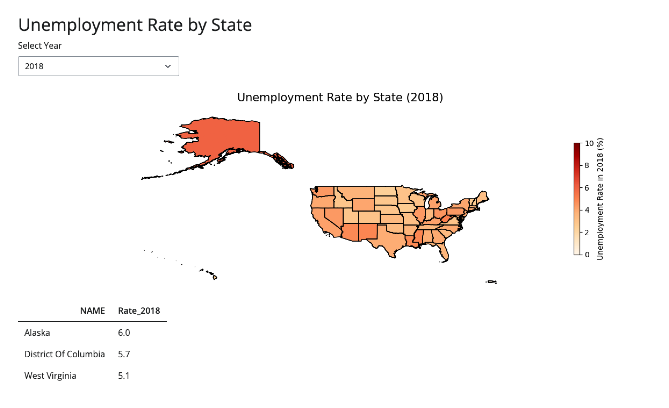
\includegraphics{finalproject_template_files/figure-pdf/cell-12-output-1.pdf}

\begin{Shaded}
\begin{Highlighting}[]
\NormalTok{image\_path\_2 }\OperatorTok{=}\NormalTok{ os.path.join(dynamic\_1\_path, }\StringTok{\textquotesingle{}p2.png\textquotesingle{}}\NormalTok{)}

\NormalTok{img\_2 }\OperatorTok{=}\NormalTok{ mpimg.imread(image\_path\_2)}
\NormalTok{plt.imshow(img\_2)}
\NormalTok{plt.axis(}\StringTok{\textquotesingle{}off\textquotesingle{}}\NormalTok{)}
\NormalTok{plt.show()}
\end{Highlighting}
\end{Shaded}

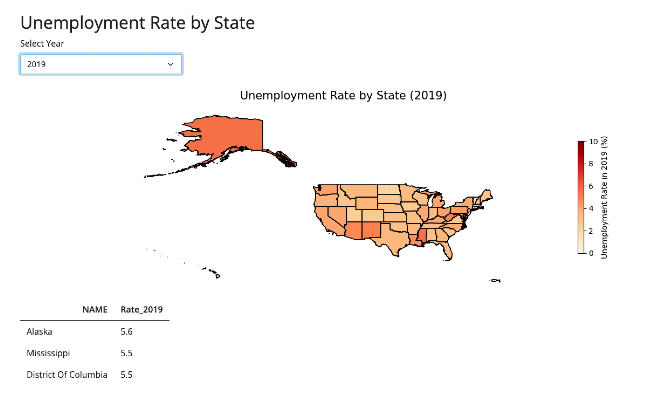
\includegraphics{finalproject_template_files/figure-pdf/cell-13-output-1.pdf}

\begin{Shaded}
\begin{Highlighting}[]
\NormalTok{image\_path\_3 }\OperatorTok{=}\NormalTok{ os.path.join(dynamic\_1\_path, }\StringTok{\textquotesingle{}p3.png\textquotesingle{}}\NormalTok{)}

\NormalTok{img\_3 }\OperatorTok{=}\NormalTok{ mpimg.imread(image\_path\_3)}
\NormalTok{plt.imshow(img\_3)}
\NormalTok{plt.axis(}\StringTok{\textquotesingle{}off\textquotesingle{}}\NormalTok{)}
\NormalTok{plt.show()}
\end{Highlighting}
\end{Shaded}

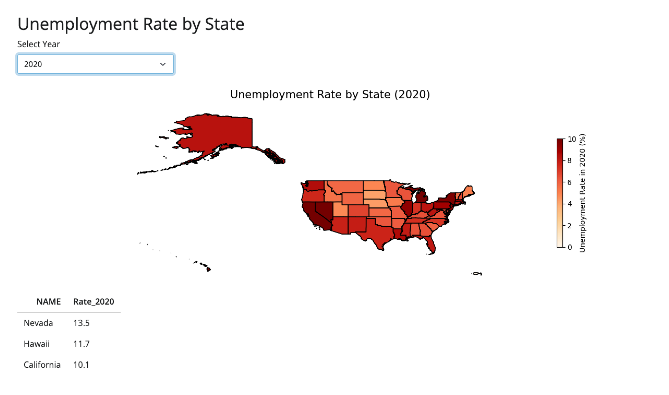
\includegraphics{finalproject_template_files/figure-pdf/cell-14-output-1.pdf}

\begin{quote}
\begin{quote}
\begin{quote}
\begin{quote}
\begin{quote}
\begin{quote}
\begin{quote}
xyz \# 4. Dynamic Trends of Real GDP and Unemployment Rate Under CARES
Act
\end{quote}
\end{quote}
\end{quote}
\end{quote}
\end{quote}
\end{quote}
\end{quote}

\begin{Shaded}
\begin{Highlighting}[]
\CommentTok{\# For a detailed view of how these figures were generated, please refer to the code in app.py. The dynamic trends presented here are the final output of our detailed data processing and visualization pipeline. }

\NormalTok{dynamic\_2\_path }\OperatorTok{=} \StringTok{\textquotesingle{}/Users/cynthia/Desktop/final{-}project{-}xy{-}wz/picture/dynamic\_2\textquotesingle{}}

\NormalTok{screenshot\_path\_1 }\OperatorTok{=}\NormalTok{ os.path.join(dynamic\_2\_path, }\StringTok{\textquotesingle{}All\_period.png\textquotesingle{}}\NormalTok{)}
\NormalTok{screenshot\_path\_2 }\OperatorTok{=}\NormalTok{ os.path.join(dynamic\_2\_path, }\StringTok{\textquotesingle{}Pre\_Cares.png\textquotesingle{}}\NormalTok{)}
\NormalTok{screenshot\_path\_3 }\OperatorTok{=}\NormalTok{ os.path.join(dynamic\_2\_path, }\StringTok{\textquotesingle{}Implementation\_period.png\textquotesingle{}}\NormalTok{)}
\NormalTok{screenshot\_path\_4 }\OperatorTok{=}\NormalTok{ os.path.join(dynamic\_2\_path, }\StringTok{\textquotesingle{}After\_Implementation.png\textquotesingle{}}\NormalTok{) }


\KeywordTok{def}\NormalTok{ show\_image(image\_path, figsize}\OperatorTok{=}\NormalTok{(}\DecValTok{10}\NormalTok{, }\DecValTok{8}\NormalTok{)):}
\NormalTok{    img }\OperatorTok{=}\NormalTok{ mpimg.imread(image\_path)}
\NormalTok{    plt.figure(figsize}\OperatorTok{=}\NormalTok{figsize)}
\NormalTok{    plt.imshow(img)}
\NormalTok{    plt.axis(}\StringTok{\textquotesingle{}off\textquotesingle{}}\NormalTok{)}
\NormalTok{    plt.show()}

\CommentTok{\# Show all the images sequentially to highlight different phases under CARES Act}
\NormalTok{show\_image(screenshot\_path\_1)}
\NormalTok{show\_image(screenshot\_path\_2)}
\NormalTok{show\_image(screenshot\_path\_3)}
\NormalTok{show\_image(screenshot\_path\_4)}
\end{Highlighting}
\end{Shaded}

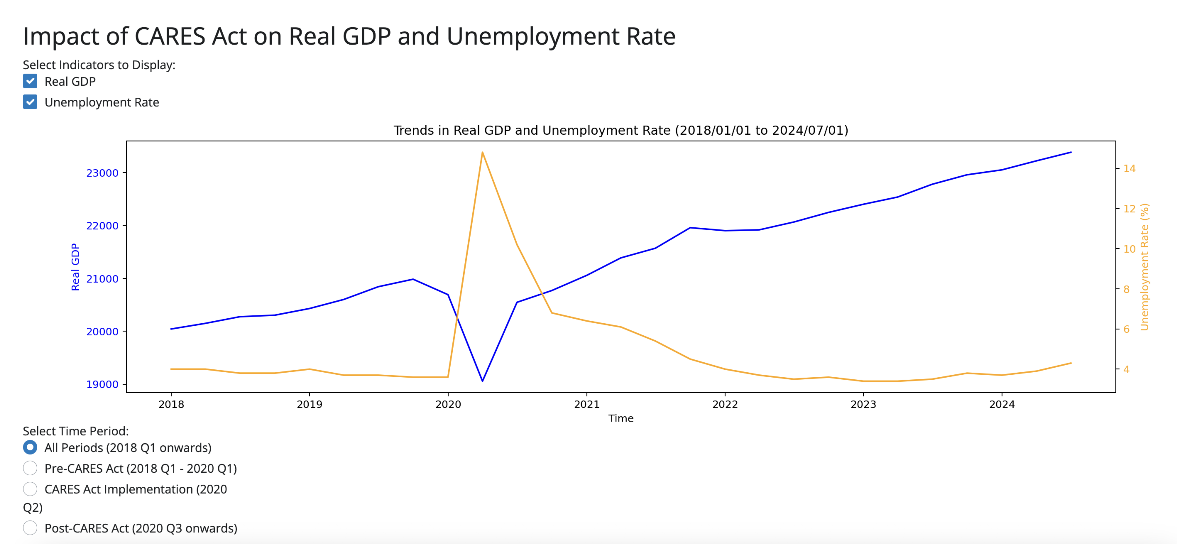
\includegraphics{finalproject_template_files/figure-pdf/cell-15-output-1.pdf}

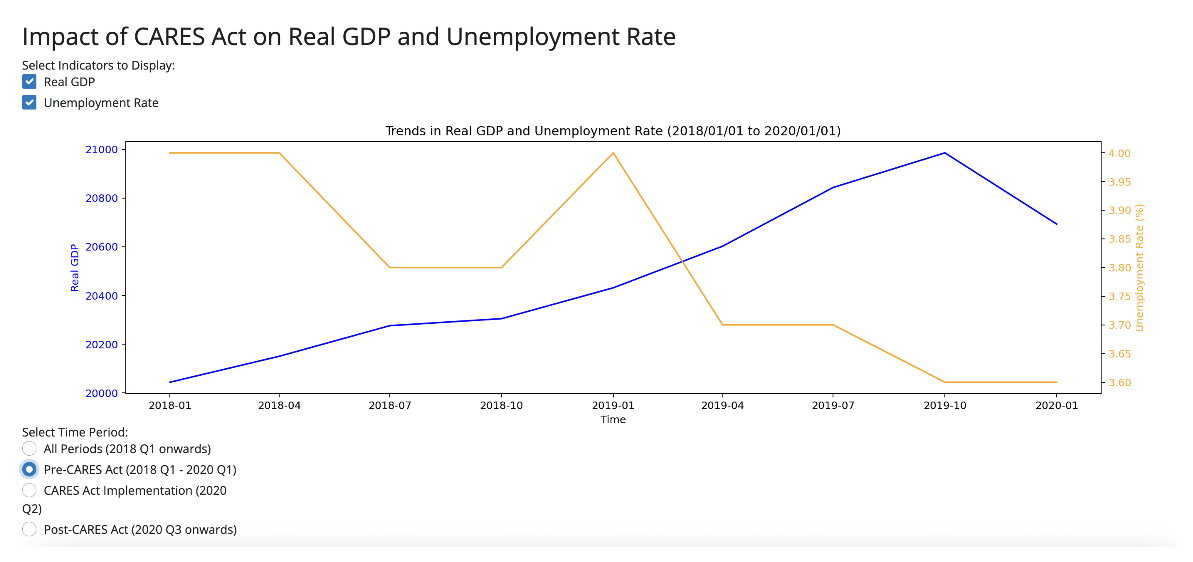
\includegraphics{finalproject_template_files/figure-pdf/cell-15-output-2.pdf}

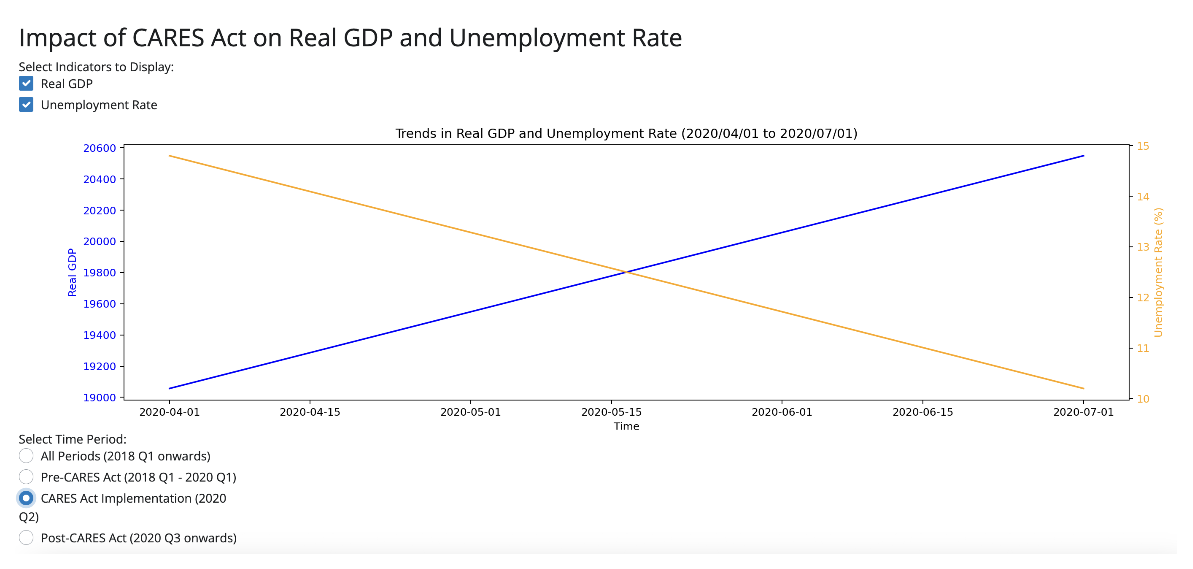
\includegraphics{finalproject_template_files/figure-pdf/cell-15-output-3.pdf}

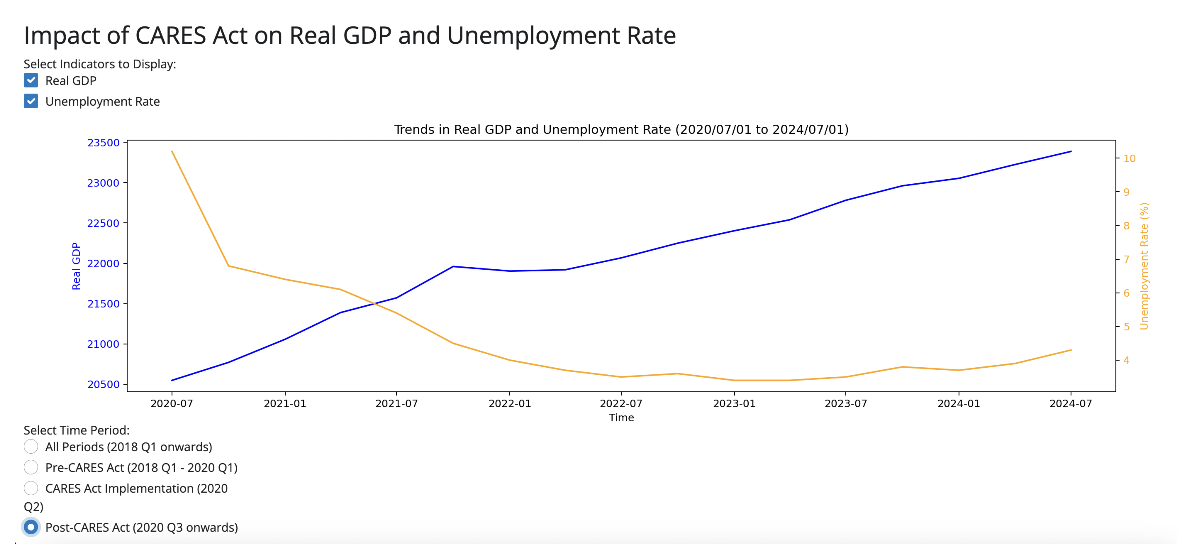
\includegraphics{finalproject_template_files/figure-pdf/cell-15-output-4.pdf}




\end{document}
